\documentclass[a4paper,titlepage]{article}
\title{Zelflerende Systemen}
\author{Steven Bronsveld en Thijs van Loenhout}

\usepackage[dutch]{babel}
\usepackage{graphicx}
\usepackage{multirow}
\usepackage{blindtext}
\usepackage{csquotes}
\usepackage{float}
\usepackage{amsmath}
\usepackage[backend=bibtex,sorting=none]{biblatex}
\usepackage{color}

\bibliography{references.bib}

\definecolor{praktijk}{rgb}{1,0.5,0}

\MakeOuterQuote{"}

\graphicspath{ {res/} }

\begin{document}



\textcolor{praktijk}{
	\section{Praktijk 1}
}


\subsection{Inleiding}
Nu wij in de vorige hoofdstukken de nodige achterliggende theorie hebben onderzocht, gaan we onze kennis inzetten voor het maken van twee praktijkopdrachten: een spel die een programma moet leren spelen en een programma om handgeschreven nummers te herkennen. In dit hoofdstuk zijn wij bezig met de vraag \textit{Welke onderdelen zijn nodig voor een zelflerend computersysteem, in de vorm van een door ons ontworpen computerprogramma, dat in staat is een eenvoudig, zelfgemaakt computerspel, met daarin meerdere obstakels, te spelen?}

\subsection{Het spel}
Voordat we het zelflerende deel van het programma kunnen maken, moet er eerst een spel komen. Hiervoor kiezen wij een \textit{platformer}. Er is een wereld waar de speler doorheen kan springen. De wereld wordt niet volgens een vast patroon gegenereerd. Er zitten heuvels, kuilen en gaten in. Wanneer de speler in zo'n gat valt, gaat deze dood. Het doel van het spel is simpelweg zo ver mogelijk te komen. Lopen doe je automatisch, dus het komt echt aan op de timing van je sprong. Voor een mens is dit makkelijk te bevatten, maar voor een computer kan dit een groot obstakel blijken te zijn.
In figuur \ref{fig:platformer1} is goed te zien hoe het spel is opgebouwd uit 'blokjes'. Op sommige blokjes, de groene, kan de speler staan. Alles wat blauw is, is niet solide en de speler valt er dus doorheen. (Dit is een eerdere versie van het spel)

\begin{figure}[h]
  \centering
    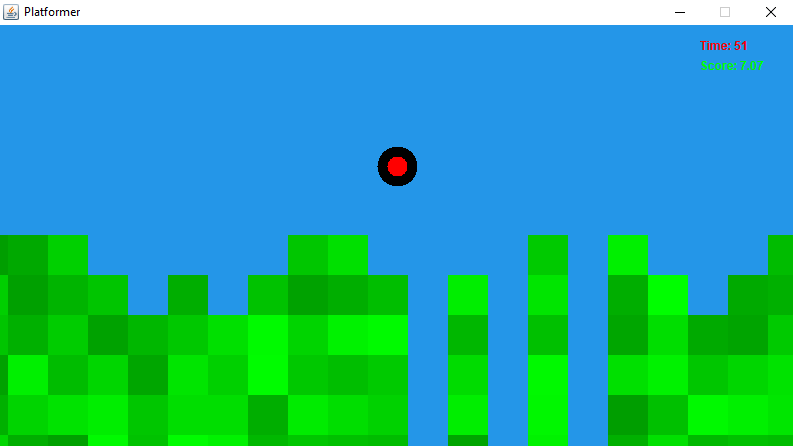
\includegraphics[width=0.5\textwidth]{platformer1.png}
  \caption{De eerste versie van het spel}
  \label{fig:platformer1}
\end{figure}

\subsection{Evolutionary improvement toepassen}
Nu is het tijd om een zelflerend systeem te maken die dit spel kan leren spelen. We doen dit met evolutionary improvement (zie hoofstuk 5). Eigenlijk moet het programma een enkele vraag kunnen beantwoorden: wat is het beste moment om te springen? 
Elk individu die het spel speelt heeft DNA. In dit DNA staat beschreven hoe lang een speler telkens moet wachten voordat hij springt. (Ook staan de kleuren van het blokje en van de ogen hierin beschreven, maar dat heeft geen invloed op het spelen van het spel) Het DNA van de best presterende individuen kan worden doorgegeven tussen generaties. Het idee is dat het programma zo steeds beter wordt doordat het steeds 'beter' DNA voor zijn spelers heeft.
Ook kunnen er willekeurige mutaties en \textit{crossovers} plaatsvinden. Een mutatie is een verandering in het DNA en een crossover is het op twee verschillende plekken wisselen van de informatie op het DNA. Deze acties worden ondernomen om diversiteit in de populatie te vergroten. Stel je voor dat je op tijdstip 1,0 moet springen, maar geen enkel individu heeft hier de code voor, dan zal er nooit vordering kunnen komen.

\begin{figure}[h]
  \centering
    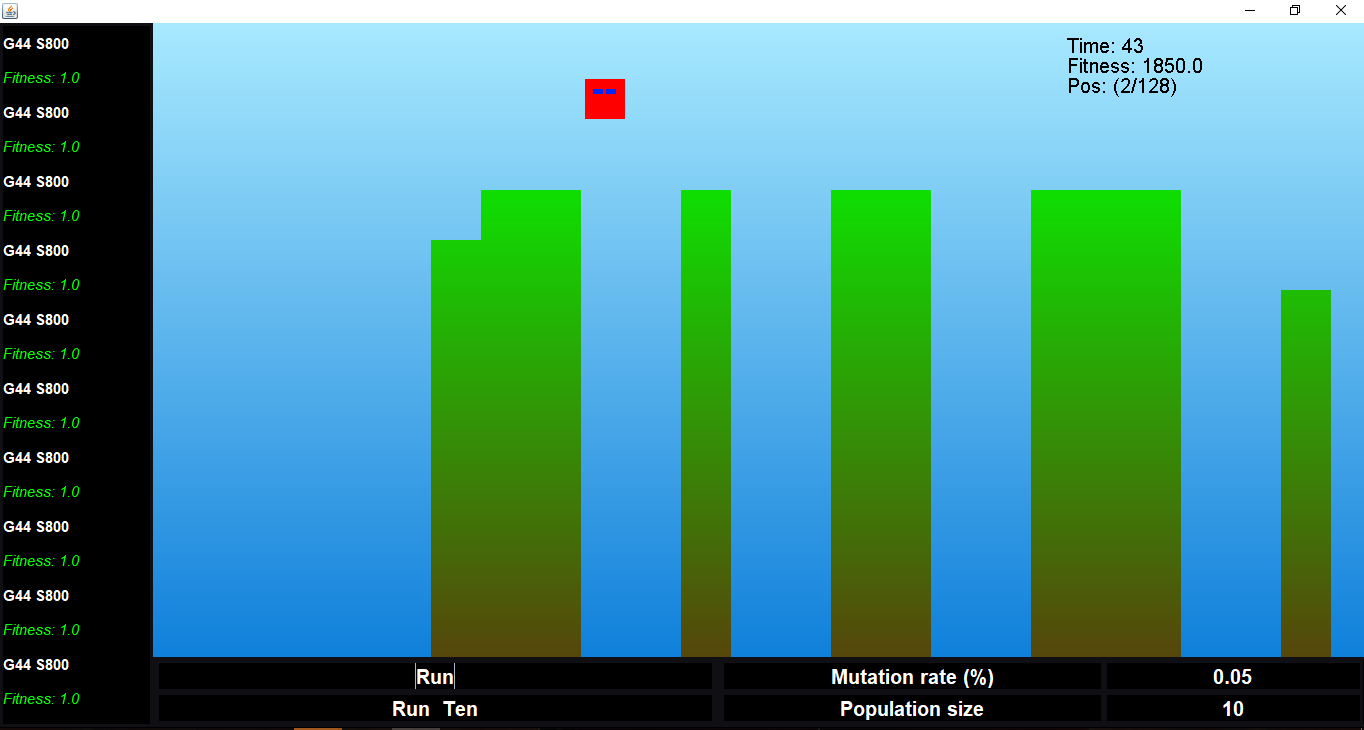
\includegraphics[width=0.5\textwidth]{platformer2.png}
  \caption{Een bepaald individu die, aangestuurd door het programma, het spel speelt}
  \label{fig:platformer1}
\end{figure}

\subsection{De resultaten}
TODO?

\subsection{Conclusie}
TODO

\end{document}
